\documentclass[notheorems,serif,table,compress]{beamer}  %dvipdfm选项是关键,否则编译统统通不过
%%------------------------常用宏包------------------------
%%注意, beamer 会默认使用下列宏包: amsthm, graphicx, hyperref, color, xcolor, 等等
\usepackage{fontspec,xunicode,xltxtra}  % for XeTeX
\usepackage{verbatim}
\usepackage{mathabx}
\usepackage{latexsym}
\usepackage{amsfonts,amssymb}
\usepackage{styles/iplouclistings}
\usepackage{fancybox}
\usepackage{colortbl}
\usepackage{tcolorbox}
%\usepackage[T1]{fontenc}
%\usepackage{bookman}
\usepackage{subfigure}
\usepackage{hyperref}
\usepackage{listings}
\usepackage{animate}
\usepackage[absolute,overlay]{textpos}
\usepackage{graphicx}
\usepackage{tikz}
\usepackage[americaninductors,europeanresistors]{circuitikz}
\usepackage{tikz}
\usepackage{fancybox}     %% 定义zhushadow时用到
\usepackage{pifont} %ding用到
\newsavebox{\mysaveboxOne}  %%为了在only中使用lstlisting
\newsavebox{\mysaveboxTwo}
\newsavebox{\mysaveboxThree}
\newsavebox{\mysaveboxFour}
\newsavebox{\mysaveboxFive}
\newsavebox{\mysaveboxSix}
\newsavebox{\mysaveboxSeven}
\newcommand\zhushadow[2][purple]{\hskip5pt\shadowbox{\color{#1}\small\kai #2\vspace{3mm}}}

%%------------------------ThemeColorFont------------------------
%% Presentation Themes
% \usetheme[<options>]{<name list>}
%\usetheme{Madrid}
\usetheme{Berkeley}
%% Inner Themes双精度计算
% \useinnertheme[<options>]{<name>}
%% Outer Themes
% \useoutertheme[<options>]{<name>}
%\useoutertheme{miniframes} 
%% Color Themes 
%\usecolortheme[<options>]{<name list>}
%% Font Themes
\usefonttheme{serif}
\setbeamertemplate{background canvas}[vertical shading][bottom=white,top=structure.fg!7] %%背景色, 上25%的蓝, 过渡到下白.
\setbeamertemplate{theorems}[numbered]
\setbeamertemplate{navigation symbols}{}   %% 去掉页面下方默认的导航条.
\usepackage{styles/zhfontcfg}
%\setsansfont[Mapping=tex-text]{文泉驿正黑}  %% 需要fontspec宏包
     %如果装了Adobe Acrobat,可在font.conf中配置Adobe字体的路径以使用其中文字体
     %也可直接使用系统中的中文字体如SimSun,SimHei,微软雅黑 等
     %原来beamer用的字体是sans family;注意Mapping的大小写,不能写错
     %设置字体时也可以直接用字体名,以下三种方式等同:
     %\setromanfont[BoldFont={黑体}]{宋体}
     %\setromanfont[BoldFont={SimHei}]{SimSun}
     %\setromanfont[BoldFont={"[simhei.ttf]"}]{"[simsun.ttc]"}
%%------------------------MISC------------------------
\graphicspath{{figures/}}         %% 图片路径. 本文的图片都放在这个文件夹里了.
%%------------------------listing------------------------
%\lstset{language=[LaTeX]TeX,Python}
%%------------------------正文------------------------
\begin{document}
\XeTeXlinebreaklocale "zh"         % 表示用中文的断行
\XeTeXlinebreakskip = 0pt plus 1pt % 多一点调整的空间
%%----------------------------------------------------------
%% This is only inserted into the PDF information catalog. Can be left
%% out.
%%%
%% Delete this, if you do not want the table of contents to pop up at
%% the beginning of each subsection:
%\AtBeginSection[]{                              % 在每个Section前都会加入的Frame
%  \frame<handout:0>{
%    \frametitle{Contents}\small
%    \tableofcontents[current,currentsubsection]
%  }
%}
%
%\AtBeginSubsection[]                            % 在每个子段落之前
%{
%  \frame<handout:0>                             % handout:0 表示只在手稿中出现
%  {
%    \frametitle{Contents}\small
%    \tableofcontents[current,currentsubsection] % 显示在目录中加亮的当前章节
%  }
%}

\setbeamertemplate{caption}{\raggedright\insertcaption\par}

%%----------------------------------------------------------
\logo{
\includegraphics[scale=0.13]{ouclogo.png}}
\title{Shape Features}
%\subtitle{Bottom-Up Saliency Detection Model Based on Human Visual Sensitivity and Amplitude Spectrum}
%\subtitle{基于边缘的图像分割}
\author[]{\textcolor{olive}{WangRuchen}}
\institute[CVBIOUC]
{
\small\textcolor{violet}{CVBIOUC\\
%Ocean University of China\\
\url{http://vision.ouc.edu.cn/~zhenghaiyong}}
}
%\date[]{}
%\titlegraphic{
%
\includegraphics[height=1.0cm]{ouc-logo.jpg}}
\frame{ \titlepage }
%%----------------------------------------------------------
%\section*{Contents}
\frame{\frametitle{Contents}\tableofcontents}
%%----------------------------------------------------------
\def\hilite<#1>{\temporal<#1>{\color{blue!15}}{\color{black}}{\color{black}}}
\newcommand{\shadow}[2][purple]{\hskip5pt\shadowbox{\color{#1}\small \kai #2\vspace{3mm}}}
\newcommand{\colorrbox}[2][purple]{\doublebox{\color{#1}\small \kai#2}}

%============================================================================

\section{Introduction}

%==========================================================================

\subsection{Why study shape?}
\begin{frame}[fragile]
\frametitle{1.1 Why study shape?}
Humans can recognize many objects based on shape alone.
    \begin{figure}
        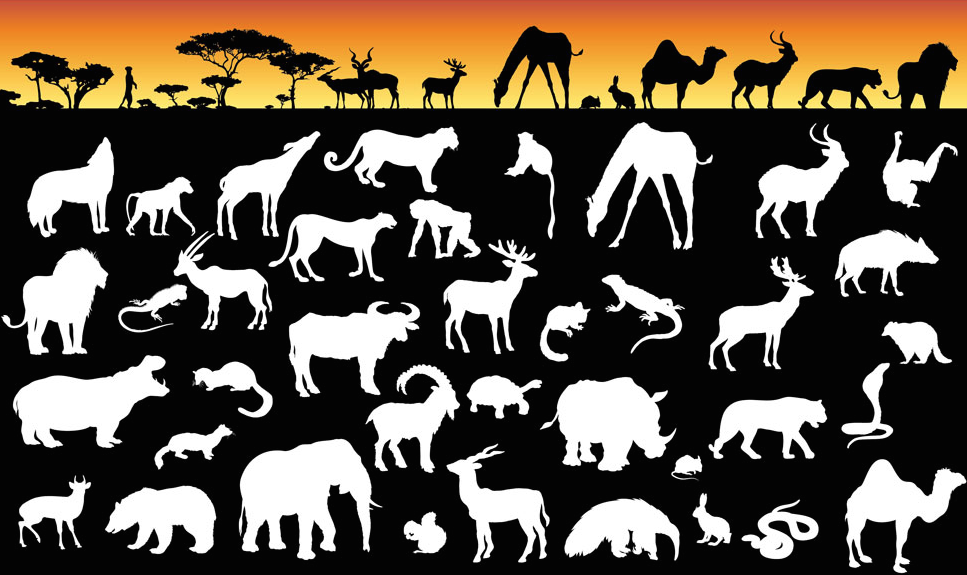
\includegraphics[width=1\linewidth]{jianying}
    \end{figure}
\end{frame}

 
\subsection{Application}

\begin{frame}
\frametitle{1.2 Application}
    \begin{itemize}
        \item Image retrieval
        \item Character recognition
        \item Object detection
        %\item Image segmentation
        \item $\dots$
    \end{itemize}
\end{frame}

\subsection{Matching \& Recognition}

\begin{frame}
\frametitle{1.3 Matching \& Recognition}
    \begin{figure}
        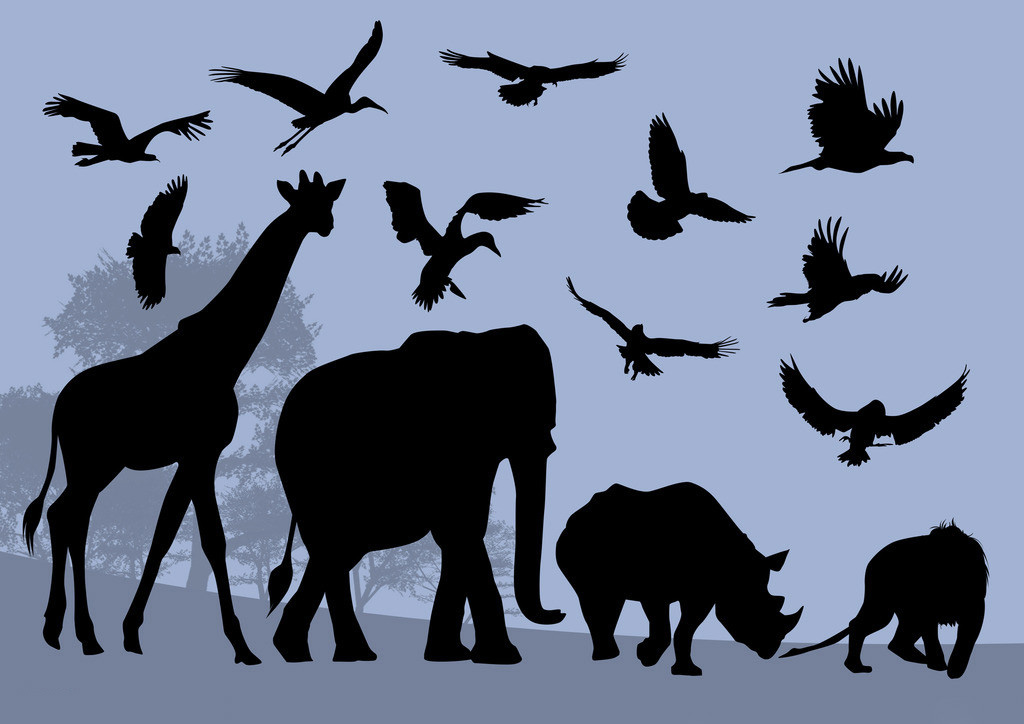
\includegraphics[width=0.5\linewidth]{reg}
    \end{figure}
    \pause
    Shape recognition:
    \begin{tcolorbox}[colback=red!5,colframe=blue!75!black]
        \begin{figure}
            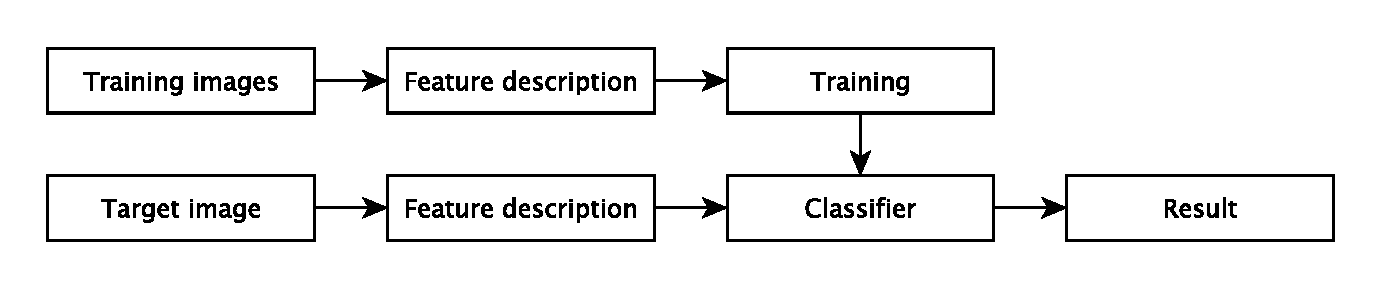
\includegraphics[width=1\linewidth]{recogChart} 
        \end{figure}
    \end{tcolorbox}
\end{frame}

\begin{frame}
\frametitle{1.3 Matching \& Recognition}
%    \begin{figure}
%        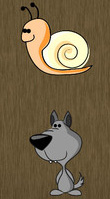
\includegraphics[width=0.55\linewidth]{match1}
%    \end{figure}
            \begin{figure}
              \centering
              \begin{minipage}[t]{0.2\linewidth}
              \centering
              
\includegraphics[width=0.6\linewidth]{match2} 
              \end{minipage}
              \pause
              \begin{minipage}[t]{0.2\linewidth}
              \centering
              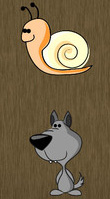
\includegraphics[width=0.6\linewidth]{match1}
              \end{minipage}
            \end{figure}
    \pause
    Shape matching:
    \begin{tcolorbox}[colback=red!5,colframe=blue!75!black]
        \begin{figure}
            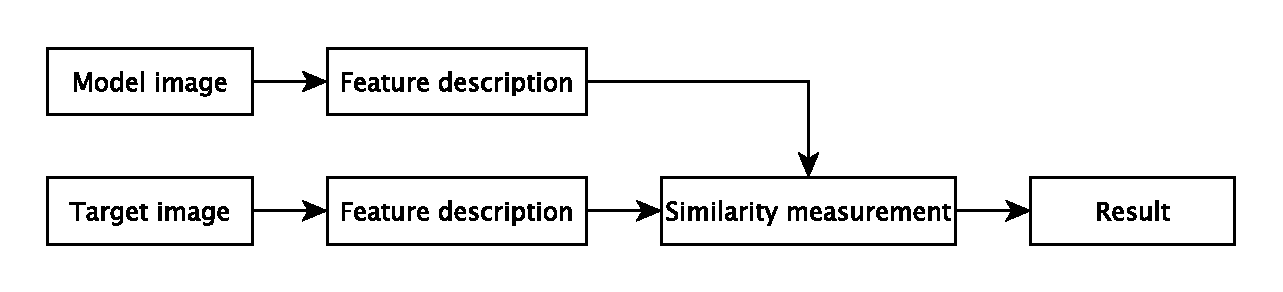
\includegraphics[width=1\linewidth]{matchChart} 
        \end{figure}
    \end{tcolorbox}
\end{frame}

\begin{frame}
\frametitle{1.3 Matching \& Recognition}
    Shape recognition:
    \begin{tcolorbox}[colback=red!5,colframe=blue!75!black]
        \begin{figure}
            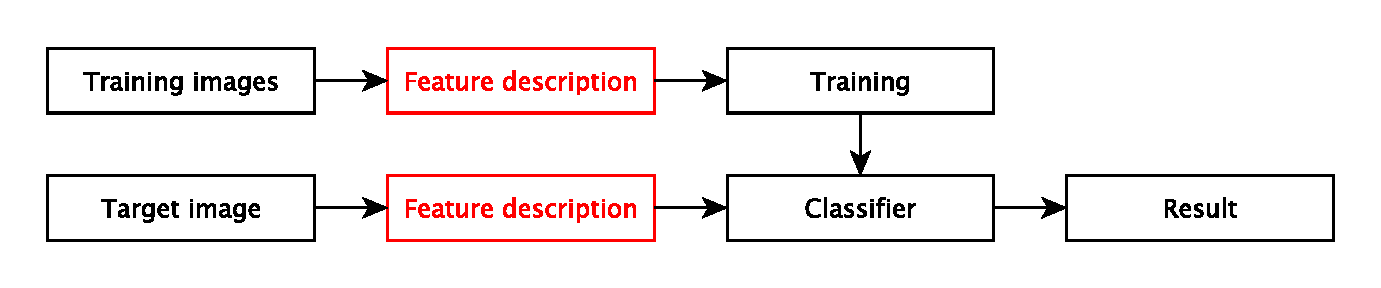
\includegraphics[width=1\linewidth]{recogChart1} 
        \end{figure}
    \end{tcolorbox}
    Shape matching:
    \begin{tcolorbox}[colback=red!5,colframe=blue!75!black]
        \begin{figure}
            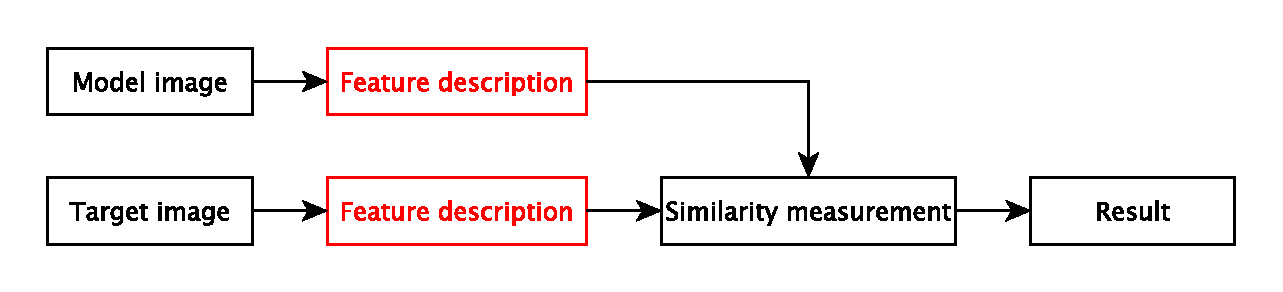
\includegraphics[width=1\linewidth]{matchChart1} 
        \end{figure}
    \end{tcolorbox}
\end{frame}


%============================================================================

\section{Shape description}

%============================================================================

\begin{frame}
\frametitle{2 Shape description}
Shape can be described in two different ways:\newline

    \begin{itemize}
        \item Contour-based\newline
        This method is connected to edge and line detection.
        \item Region-based\newline
        This method is linked to the region segmentation.
    \end{itemize}
\end{frame}

\subsection{Shape description techniques}
\begin{frame}
\frametitle{2.1 Shape description techniques\footnote{Mingqiang Yang, Kidiyo Kpalma, Joseph Ronsin. ``A Survey of Shape Feature Extraction Technique'', PR, 2010.}\footnote{Dengsheng Zhang, Guojun Lu. ``Review of shape representation and description techniques'', PR, 2003.}\footnote{Yu Zhou, Juntao Liu, Xiang Bai. ``Research and Perspective on Shape Matching'', Acta Automatica Sinica, 2012.}}
    \begin{columns}
        \begin{column}{0.55\linewidth}
            \begin{itemize}
                \item Chain code
                \item Polygonal approximation
                \item B-spline
                \item Wavelet descriptor
                \item Fourier descriptor
                \item Curvature scale space
                \item Shape context\newline
                $\dots$
                \end{itemize}
        \end{column}
        \begin{column}{0.45\linewidth}
 %       \item Chord distribution
             \begin{itemize}
                \item Skeletons
                \item Convex hull
                \item Geometric moments
                \item Zernike moments
                \item Shape matrix
                \item Core\newline
                $\dots$
            \end{itemize}
        \end{column}
    \end{columns}\vspace{1ex}
\end{frame}

\begin{frame}
\frametitle{2.1 Shape description techniques}
    \begin{itemize}
        \item Skeleton
        \item Convex hull
        \item Shape context
    \end{itemize}
\end{frame}

\subsection{Skeleton}

\begin{frame}
\frametitle{2.2 Skeleton (Medial axis)}
~~~~~~Skeleton is defined by {\color{blue}Grassfire Model}\footnote{Harry Blum. ``Biological shape and visual science'', Theoretical Biology, 1973.}. It is also defined as the locus of centers of maximal disks that 􏰁fit within the shape.    
%It can be employed for shape representation and description.
            \begin{figure}
              \centering
              \begin{minipage}[t]{0.4\linewidth}
              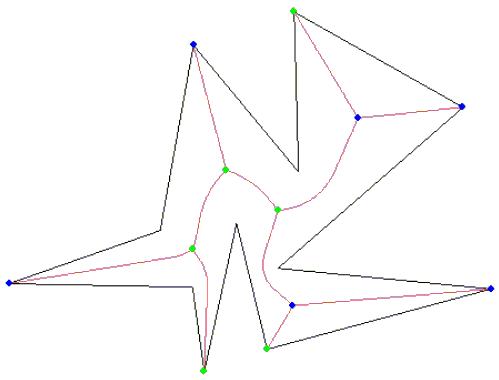
\includegraphics[width=1\linewidth]{gu} 
              \end{minipage}
              \begin{minipage}[t]{0.28\linewidth}
              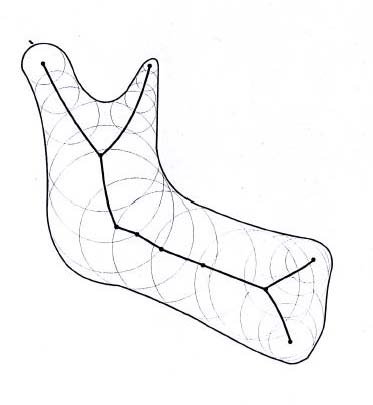
\includegraphics[width=1\linewidth]{mat1}
              \end{minipage}
            \end{figure}
\end{frame}

\subsubsection{Skeleton extraction}
\begin{frame}
\frametitle{2.2.1 Skeleton extraction (Medial axis transform)}
%~~~~~~Skeleton Extraction can get the features and topological structure of shape.\newline
%Points, which have more than one nearest points, are skeleton.
            \begin{figure}
              \centering
              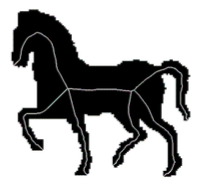
\includegraphics[width=0.4\linewidth]{skeleton} 
            \end{figure}
    \begin{itemize}
        \item Voronoi diagram
        %\item Image thinning
        \item Distance transform
        \item Mathematical morphology
    \end{itemize}
\end{frame}

\begin{frame}
\frametitle{2.2.1 Skeleton extraction \\ \normalsize{Mathematical morphology}}
    \begin{itemize}
        \item Dilation
           \begin{displaymath}
             A \oplus B= \{z|(B)_{z}\cap A\ne \oslash\}
           \end{displaymath} 
           \begin{figure}
              \centering
              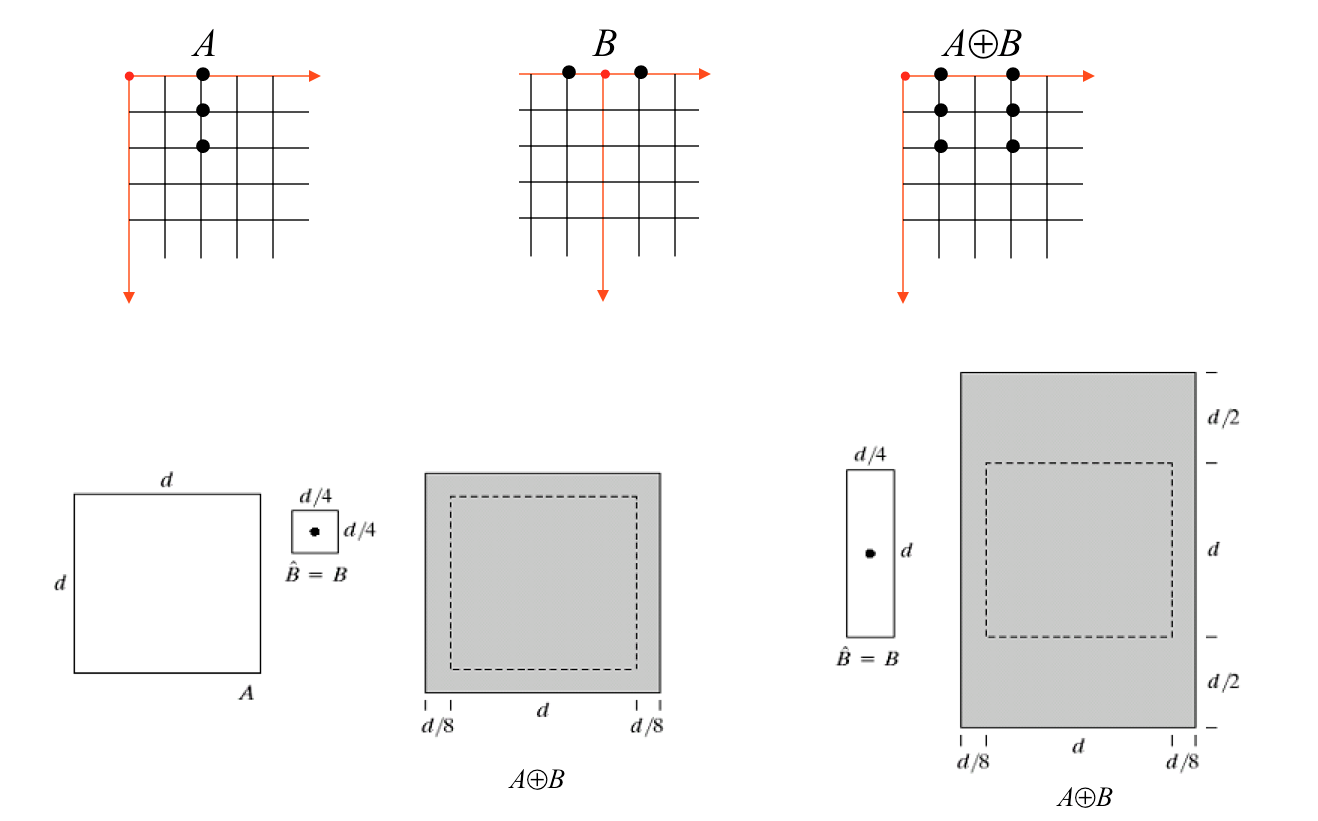
\includegraphics[width=0.7\linewidth]{dil} 
            \end{figure}
    \end{itemize}
\end{frame}

\begin{frame}
\frametitle{2.2.1 Skeleton extraction \\ \normalsize{Mathematical morphology}}
    \begin{itemize}
        \item Erosion
           \begin{displaymath}
             A \odot B= \{z|(B)_{z}\subseteq A\}
           \end{displaymath} 
            \begin{figure}
              \centering
              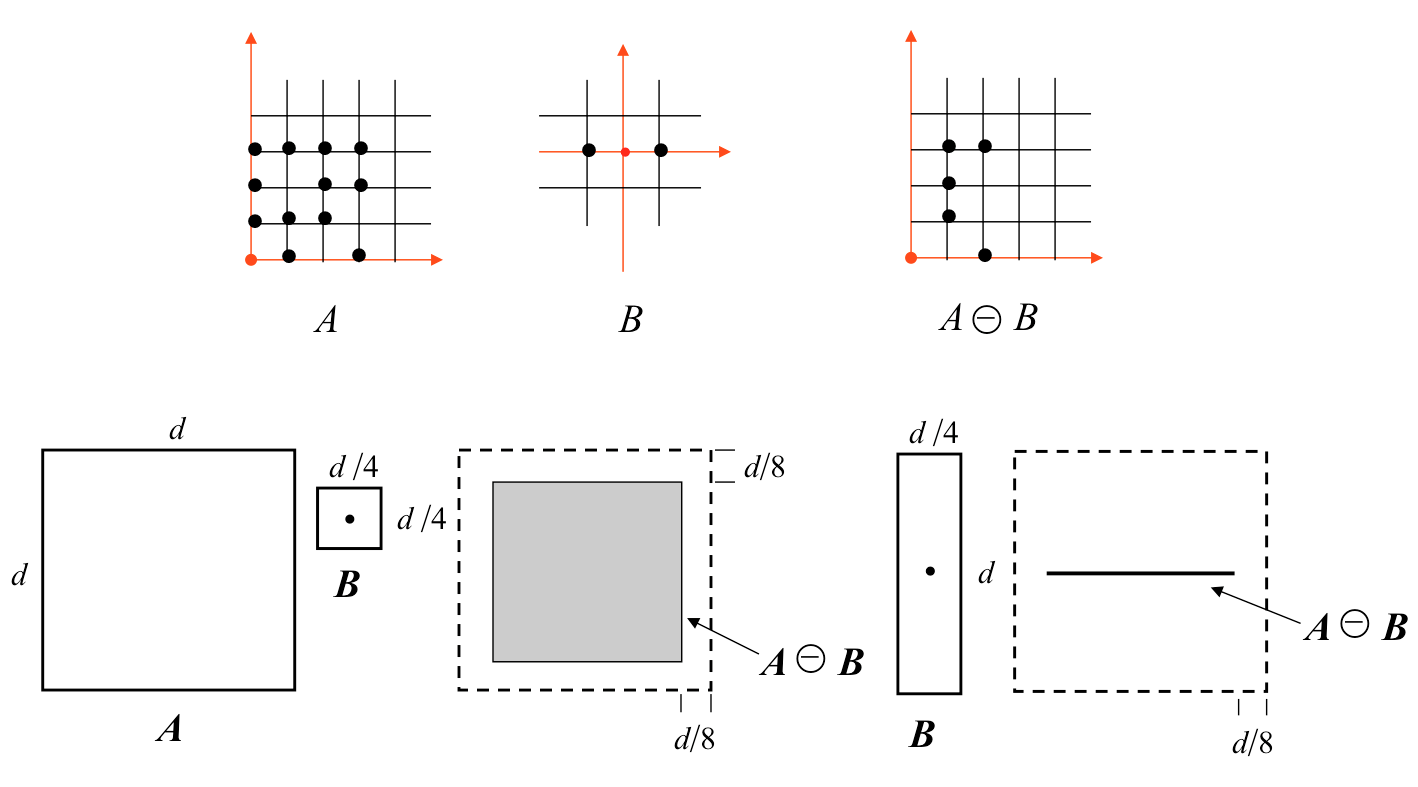
\includegraphics[width=0.7\linewidth]{ero} 
            \end{figure}
    \end{itemize}
\end{frame}

\begin{frame}
\frametitle{2.2.1 Skeleton extraction \\ \normalsize{Mathematical morphology}}
            \begin{figure}
              \centering
              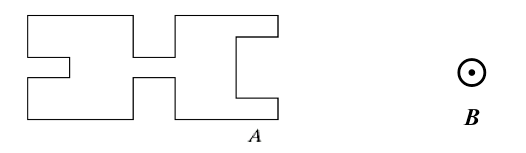
\includegraphics[width=0.35\linewidth]{yuan} 
            \end{figure}
    \begin{itemize}
        \item Opening
           \begin{displaymath}
             A \circ B=(A \odot B)\oplus B
           \end{displaymath} 
           \begin{figure}
              \centering
              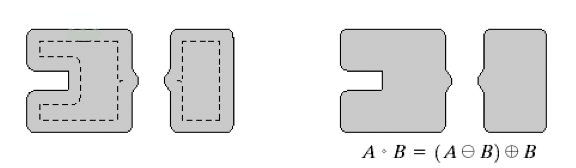
\includegraphics[width=0.52\linewidth]{open} 
            \end{figure}
        \item Closing
            \begin{displaymath}
             A \bullet B=(A \oplus B)\odot B
           \end{displaymath} 
           \begin{figure}
              \centering
              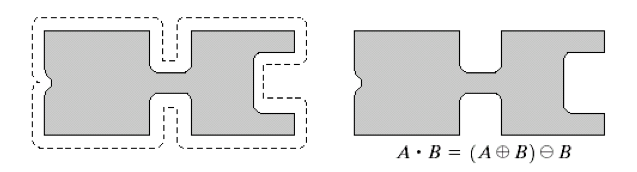
\includegraphics[width=0.52\linewidth]{close} 
            \end{figure}
    \end{itemize}
\end{frame}

\begin{frame}
\frametitle{2.2.1 Skeleton extraction \\ \normalsize{Skeletonization via Mathematical morphology}}
            \begin{figure}
              \centering
              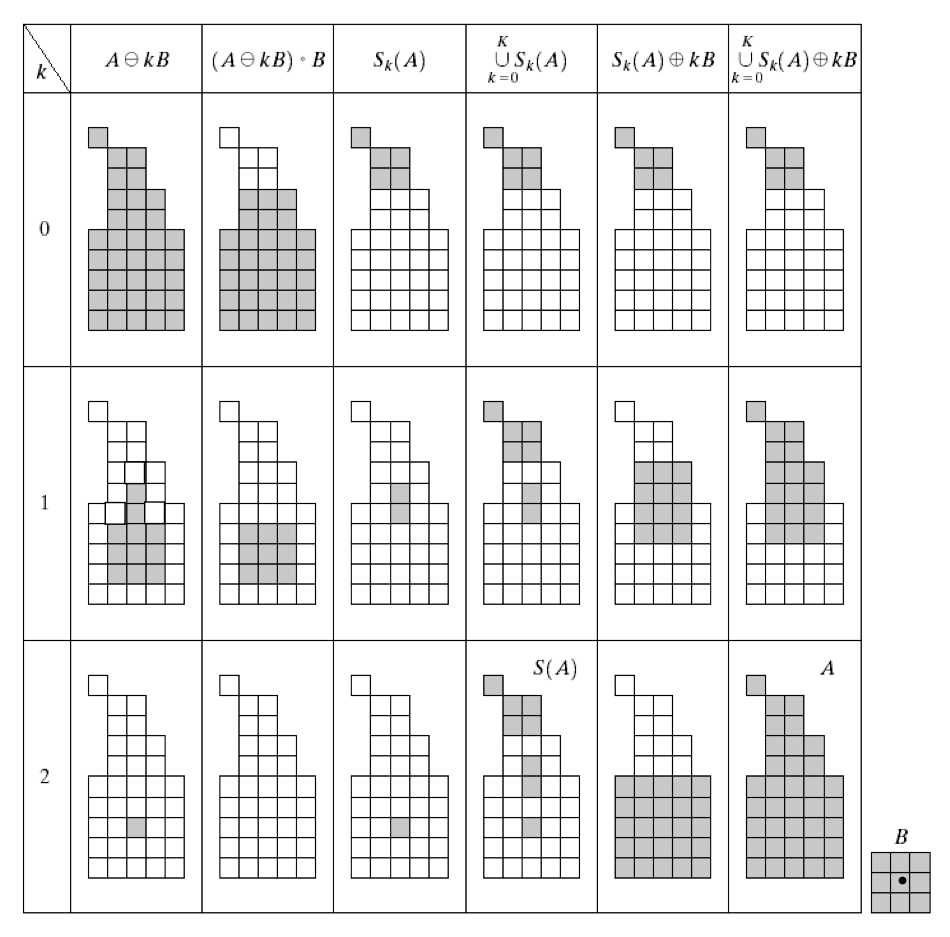
\includegraphics[width=0.7\linewidth]{xingtai} 
            \end{figure}
\end{frame}

\begin{frame}
\frametitle{2.2.1 Skeleton extraction \\ \normalsize{Skeletonization via Mathematical morphology}}
~~~~~~The skeleton of a set can be expressed in terms of erosions and openings:
           \begin{displaymath}
             S_{k}(A)=(A\ominus kB)-(A \ominus kB)\circ B
           \end{displaymath} 
            \begin{displaymath}
             S(A)=\bigcup_{k=0}^{K}S_{k(A)}
           \end{displaymath}
\begin{itemize}
\item B - is a sturcturing element.
\item K - is the last iterative step before A erodes to an empty set.
\end{itemize}
~~~~~~A can be reconstructed from its skeleton subsets $S_{k}(A)$ using the equation:
            \begin{displaymath}
             A=\bigcup_{k=0}^{K}(S_{k(A)}\oplus kB)
           \end{displaymath}
\end{frame}

\subsubsection{Attributed relation graphs}
\begin{frame}
\frametitle{2.2.2 Attributed relation graphs (ARG)}
            \begin{figure}
              \centering
              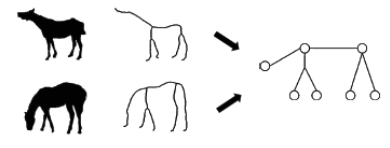
\includegraphics[width=0.5\linewidth]{gujia} 
            \end{figure}
    \begin{itemize}
        \item Shock graph\footnote{Kaleem Siddiqi \textit{et al.}. ``Shock graph and shape matching'', IJCV, 1999.}
        \item Skeleton tree\footnote{Wenyu Liu, Juntao Liu. ``Objects similarity measure based on skeleton tree descriptor matching'', Journal Infrared Millimeter and Wave, 2005.}
        \item Bone graph\footnote{Diego Macrini, Kaleem Siddiqi \textit{et al.}. ``From skeletons to bone graphs: medial abstraction for object recognition'', CVPR, 2008.}
    \end{itemize}
\end{frame}

\begin{frame}
\frametitle{2.2.2 Attributed relation graphs (ARG) \\ \normalsize{Shock graph\footnote{K Siddiqi. ``Shock graph and shape matching'', IJCV, 1999.}}}
%{\color{blue}Shock graph}:
What is shock graph?
            \begin{figure}
              \centering
              \begin{minipage}[t]{0.3\linewidth}
              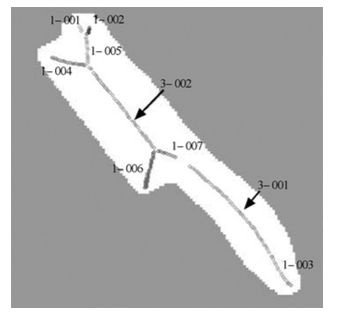
\includegraphics[width=1\linewidth]{shock2} 
              \end{minipage}
              \begin{minipage}[t]{0.3\linewidth}
              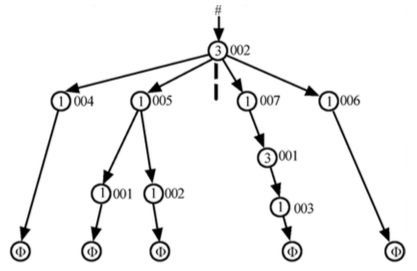
\includegraphics[width=1.4\linewidth]{shock3}
              \end{minipage}
            \end{figure}
{\color{blue}Shock points}: %four types
            \begin{figure}
              \centering
              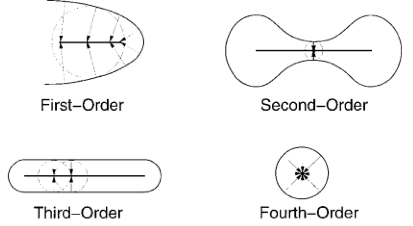
\includegraphics[width=0.4\linewidth]{shock1} 
            \end{figure}
\end{frame}

\begin{comment}
\begin{frame}
\frametitle{2.2.2 Attributed relation graphs (ARG) \\ \normalsize{Shock graph}}
{\color{blue}Shock graph grammar}:
            \begin{figure}
              \centering
              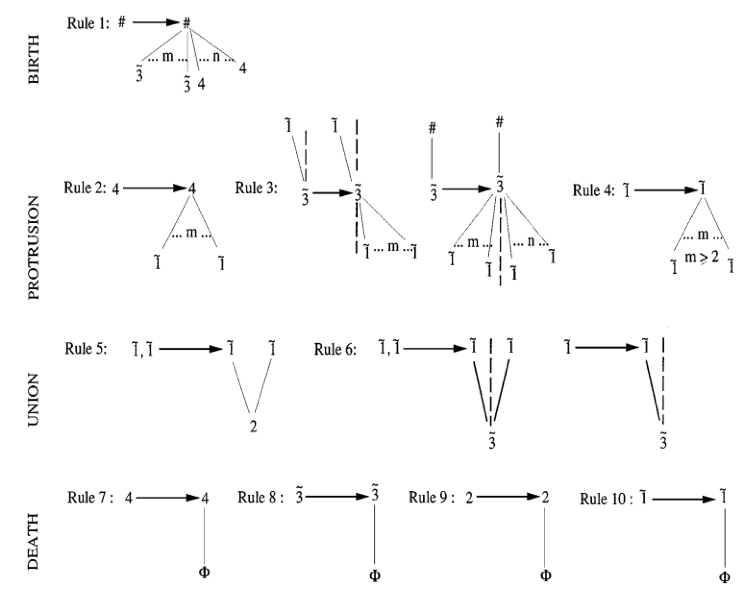
\includegraphics[width=0.7\linewidth]{gram} 
            \end{figure}
\end{frame}
\end{comment}

\begin{frame}
\frametitle{2.2.2 Attributed relation graphs (ARG) \\ \normalsize{Skeleton tree\footnote{Wenyu Liu, Juntao Liu. ``Objects similarity measure based on skeleton tree descriptor matching'', Journal Infrared Millimeter and Wave, 2005.}}}
%The skeleton can then be decomposed into segments and represented as a graph according to certain criteria. The matching between shapes becomes a graph matching. 
What is skeleton tree?% is another form.
            \begin{figure}
              \centering
              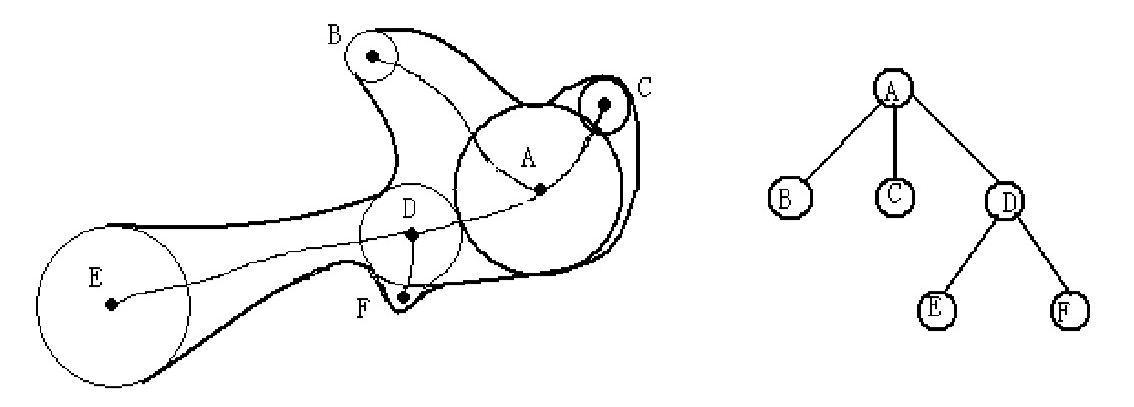
\includegraphics[width=0.6\linewidth]{tree} 
            \end{figure}
            \centering Tree descriptor: $(3,0,0,2,0,0)$
\end{frame}

\subsection{Convex hull}

\begin{frame}        
\frametitle{2.3 Convex hull}
    \begin{columns}
        \begin{column}{0.4\linewidth}
{\color{blue}What?}\newline

~~~~~~The convex hull of a region is the smallest convex polygon that contains all the points of the region.
        \end{column}
        \begin{column}{0.6\linewidth}
            \begin{tcolorbox}[colback=red!5,colframe=blue!75!black]
            \begin{figure}
              \centering
              \begin{minipage}[t]{0.32\linewidth}
              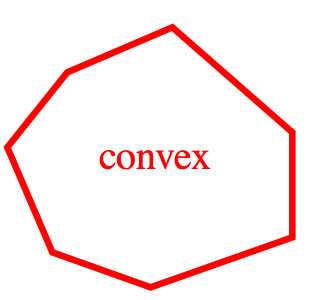
\includegraphics[width=1.1\linewidth]{hull1}
              \end{minipage}
              \begin{minipage}[t]{0.3\linewidth}
              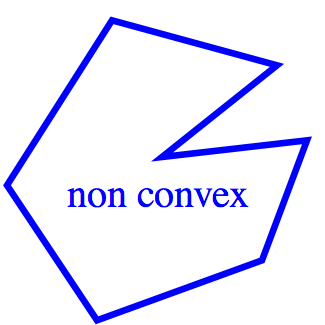
\includegraphics[width=1.1\linewidth]{hull2}
              \end{minipage}
            \end{figure}
            \begin{figure}
              \centering
              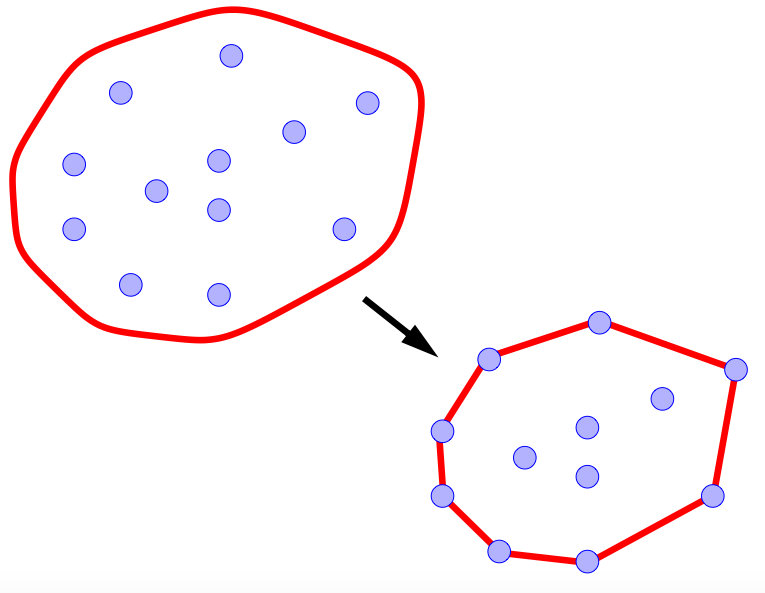
\includegraphics[width=0.6\linewidth]{hull} 
            \end{figure}
            \end{tcolorbox}
          \end{column}
    \end{columns}\vspace{1ex}
\end{frame}

\begin{frame}
\frametitle{2.3 Convex hull}
{\color{blue}How to describe shape?}
            \begin{figure}
              \centering
              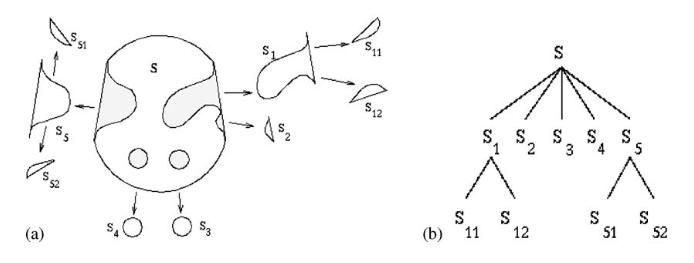
\includegraphics[width=0.7\linewidth]{hulltree} 
            \end{figure}
    \pause
{\color{blue}Convex hull algorithms}:
    \begin{itemize}
        \item Graham Scan Algorithm
        \item Quickhull Algorithm
 %       \item 
    \end{itemize}
\end{frame}

%\subsubsection{}
\begin{frame}
\frametitle{2.3 Convex hull}
    \begin{itemize}
        %\item Gift Wrapping Algorithm
        \item Graham Scan Algorithm\footnote{Ronald L. Graham. ``An Efficient Algorithm for Determining the Convex Hull of a Finite Planar Set'', Information Processing Letters, 1972.}
            \begin{figure}
              \centering
              \begin{minipage}[t]{0.35\linewidth}
              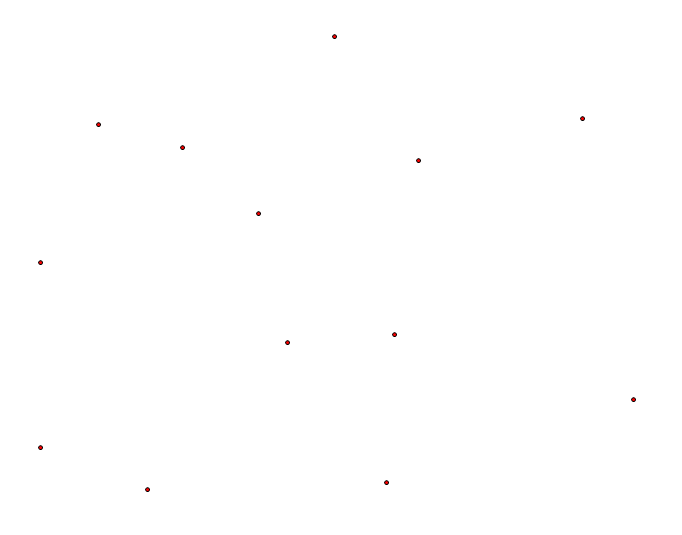
\includegraphics[width=1\linewidth]{gra1}
              \end{minipage}
              \pause
              \begin{minipage}[t]{0.35\linewidth}
              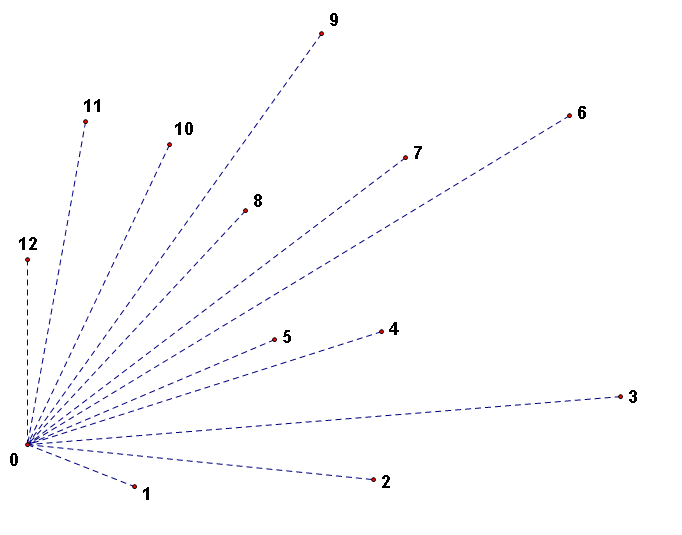
\includegraphics[width=1\linewidth]{gra2}
              \end{minipage}
            \end{figure}
            \pause
            \begin{figure}
              \centering
              \begin{minipage}[t]{0.35\linewidth}
              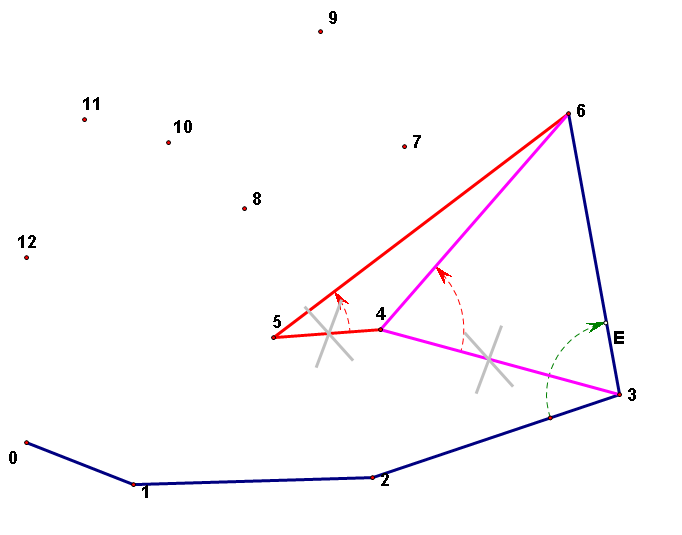
\includegraphics[width=1\linewidth]{gra3}
              \end{minipage}
              \pause
              \begin{minipage}[t]{0.35\linewidth}
              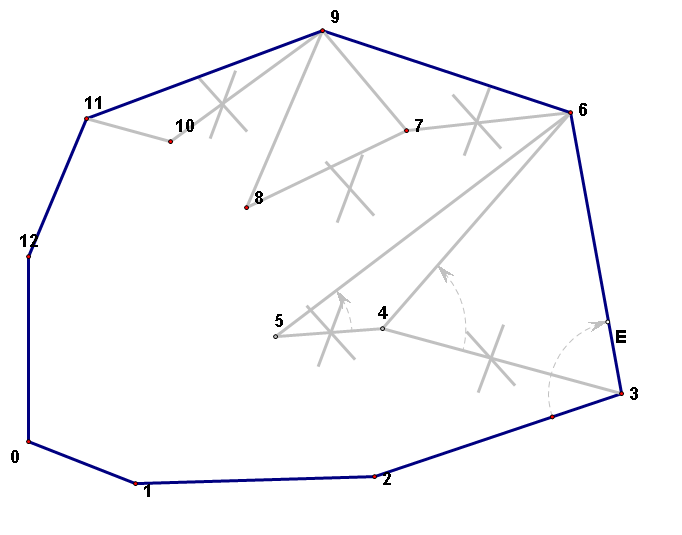
\includegraphics[width=1\linewidth]{gra4}
              \end{minipage}
            \end{figure}
    \end{itemize}
\end{frame}

\begin{frame}
\frametitle{2.3 Convex hull}
    \begin{itemize}
        \item Quickhull Algorithm\footnote{Barber C. Bradford \textit{et al.}. ``The quickhull algorithm for convex hulls'', ACM Transactions on Mathematical Software, 1996.}
        \begin{figure}
              \centering
              \begin{minipage}[t]{0.35\linewidth}
              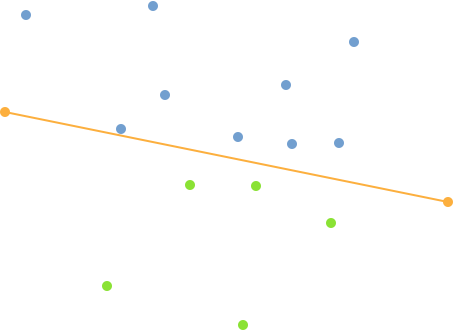
\includegraphics[width=1\linewidth]{quick1}
              \end{minipage}
              \pause
              \begin{minipage}[t]{0.35\linewidth}
              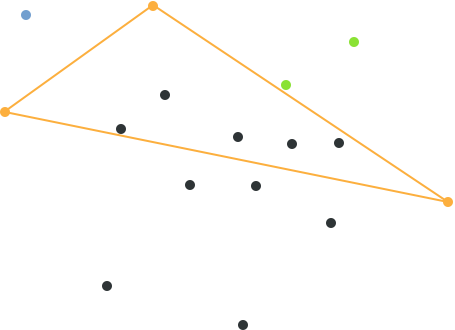
\includegraphics[width=1\linewidth]{quick2}
              \end{minipage}
        \end{figure}
        \pause
        \begin{figure}
              \centering
              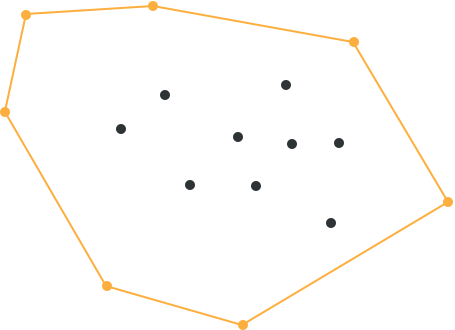
\includegraphics[width=0.35\linewidth]{quick3} 
        \end{figure}
%            \begin{figure}
%              \centering
%              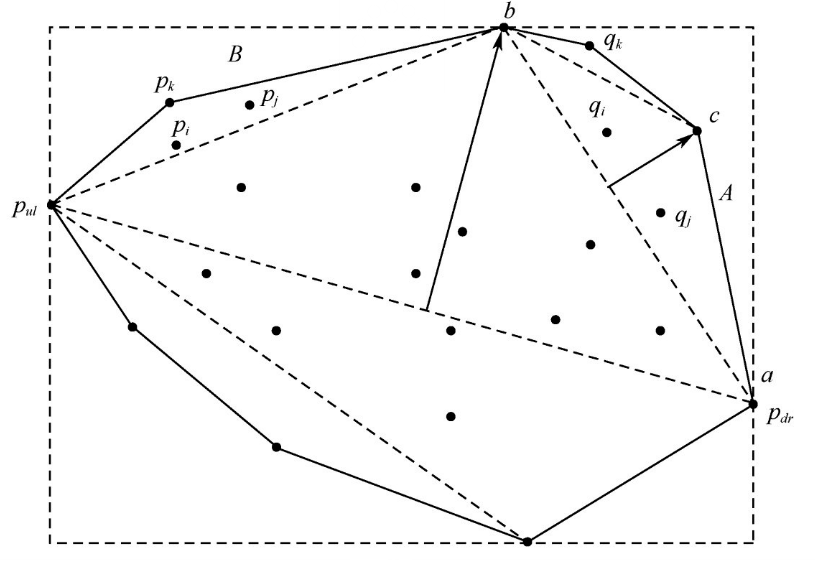
\includegraphics[width=0.5\linewidth]{hullquick}
 %           \end{figure}
    \end{itemize}
\end{frame}

\subsection{Shape context}

\begin{frame}        
\frametitle{2.4 Shape context\footnote{Serge Belongie \textit{et al.}. ``Shape Matching and Object Recognition Using Shape Contexts'', PAMI, 2002.}}
~~~~~~The shape context is intended to be a way of describing shapes that allows for measuring shape similarity and the recovering of point correspondences.\newline
%Shape context is to describe the coarse arrangement of the shape with respect to a point on the boundary of the shape.

{\color{blue}How to describe a shape?}
            \begin{figure}
              \centering
              
\includegraphics[width=0.3\linewidth]{a1}
            \end{figure}
%        \begin{figure}
%        
\includegraphics[width=0.7\linewidth]{context1.png} 
%        \end{figure}
\end{frame}

\subsubsection{How to describe a shape?}
\begin{frame}        
\frametitle{2.4.1 How to describe a shape?}
    \begin{enumerate}
        \begin{columns}
        \begin{column}{0.5\linewidth}
        \centering
        \item Obtain contours using \newline
        edge detector
            \begin{figure}
              %\centering
              
\includegraphics[width=0.4\linewidth]{a-edge}
            \end{figure}
            \end{column}
        \begin{column}{0.5\linewidth}
        \pause
        \item Pick n points on the contours of a shape
            \begin{figure}
              %\centering
              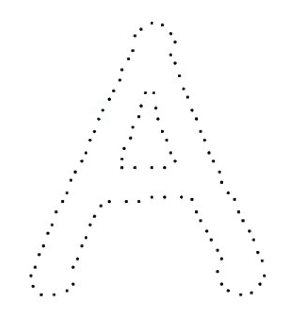
\includegraphics[width=0.4\linewidth]{a-point}
            \end{figure}
        \end{column}
    \end{columns}\vspace{1ex}
    \pause
        \item Compute the shape context of each point
            \begin{figure}
              \centering
              \begin{minipage}[t]{0.3\linewidth}
              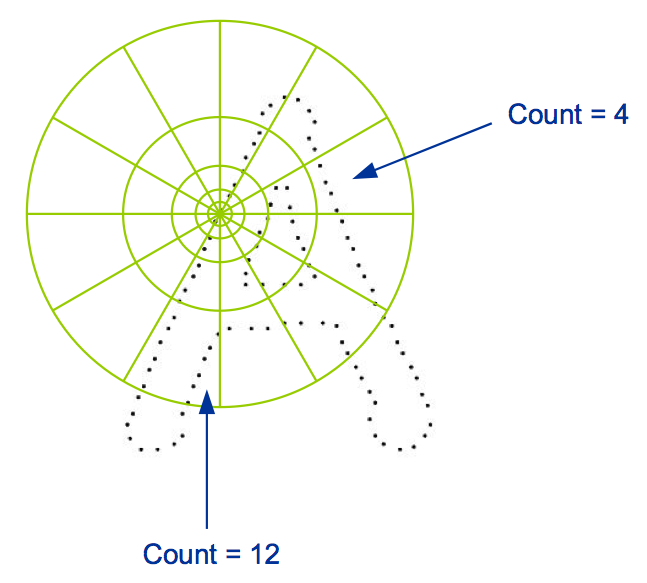
\includegraphics[width=1\linewidth]{a-log}
              \end{minipage}
              \begin{minipage}[t]{0.3\linewidth}
              \centering
              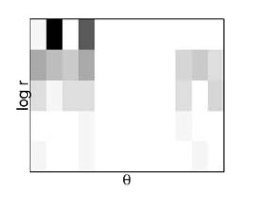
\includegraphics[width=1\linewidth]{his}
              \end{minipage}
            \end{figure}
       \end{enumerate}
\end{frame}

\subsubsection{Matching with shape contexts}
\begin{frame}
\frametitle{2.4.2 Matching with shape contexts}
            \begin{figure}
              \centering
              
\includegraphics[width=0.35\linewidth]{context1}
            \end{figure}
    \begin{itemize}
        \item Match each point from the known shape to a point on an unknown shape
    \end{itemize}
        \begin{figure}
        
\includegraphics[width=0.35\linewidth]{pointmatch} 
        \end{figure}
\end{frame}

\begin{frame}
\frametitle{2.4.2 Matching with shape contexts}
\begin{enumerate}
    \item Computing the cost matrix
    \begin{displaymath}
         C_{ij}=\frac{1}{2}\sum_{k=1}^{K}\frac{[h_{i}(k)-h_{j}(k)]^{2}}{h_{i}(k)+h_{j}(k)}
       \end{displaymath}
       $C_{ij}=C(p_{i},q_{j})$ denote the cost of matching these two points.\newline
   {\color{blue}Cost matrix}:
        \begin{displaymath}
        \left( \begin{array}{cccc}
        C_{11} & C_{12} & \ldots & C_{1n} \\
        C_{21} & C_{22} & \ldots & C_{2n} \\
        \vdots & \vdots & \ddots & \vdots \\
        C_{n1} & C_{n2} & \ldots & C_{nn}
        \end{array} \right)
        \end{displaymath}
    \item Finding the matching that minimizes total cost:
        \begin{displaymath}
        H(\pi)=\sum_{i}C(p_{i},q_{\pi(i)})
        \end{displaymath}
    \end{enumerate}
\end{frame}


\begin{frame}
\frametitle{2.4.2 Matching with shape contexts \\ \normalsize{Hungary algorithm\footnote{Harold W. Kuhn. ``The Hungarian Method for the assignment problem'', Naval Research Logistics Quarterly, 1955.}}}
Hungarian Algorithm is used in optimizing the assignment problems.\newline

\begin{itemize}
    \item Bipartite graph
\end{itemize}
    \begin{figure}
    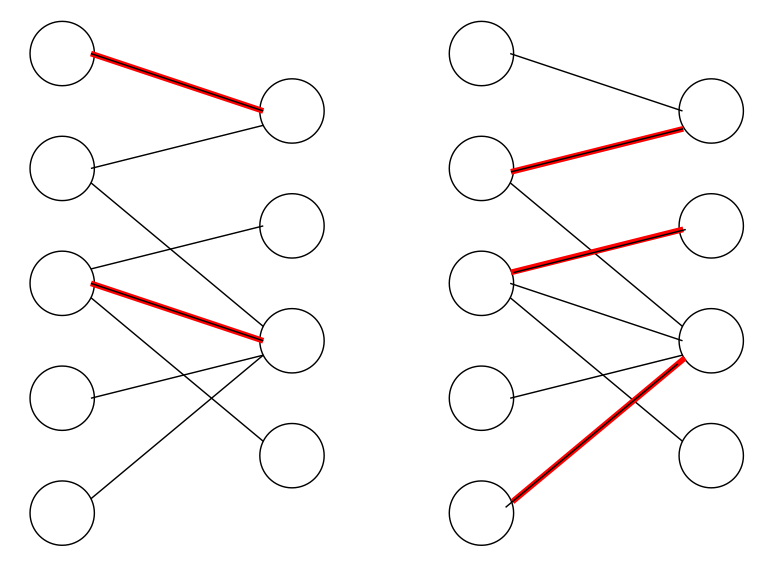
\includegraphics[width=0.5\linewidth]{xiong} 
    \end{figure}
\end{frame}

\begin{frame}
\frametitle{2.4.2 Matching with shape contexts \\ \normalsize{Hungary algorithm}}
\begin{itemize}
    \item Matrix interpretation
\end{itemize}
\flushleft
\newtheorem*{mur}{Theorem}
\begin{mur}
\footnotesize{If a number is added to or subtracted from all of the entries of any one row or column of a cost matrix, then on optimal assignment for the resulting cost matrix is also an optimal assignment for the original cost matrix.}
\end{mur}
\begin{description}
    \item[\footnotesize{Step 1.}]  \footnotesize{Subtract the smallest entry in each row from all the entries of its column.}
        \begin{figure}
        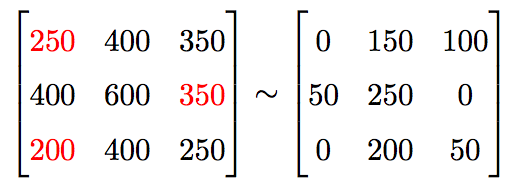
\includegraphics[width=0.4\linewidth]{1} 
        \end{figure}
    \item[Step 2.] \footnotesize{Subtract the smallest entry in each column from all the entries of its column.}
        \begin{figure}
        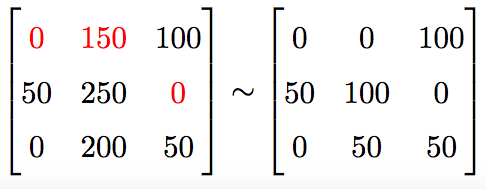
\includegraphics[width=0.4\linewidth]{2} 
        \end{figure}
\end{description}
\end{frame}

\begin{frame}
\frametitle{2.4.2 Matching with shape contexts \\ \normalsize{Hungary algorithm}}
\begin{description}
    \item[\footnotesize{Step 3.}] \footnotesize{Draw lines through appropriate rows and columns so that all the zero entries of the cost matrix are covered and the minimum number of such lines is used.}
        \begin{figure}
        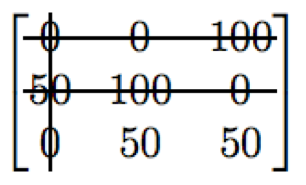
\includegraphics[width=0.24\linewidth]{3} 
        \end{figure}
    \item[Step 4.] \footnotesize{(i)If the minimum number of covering lines is n, an optimal assignment of zeros is possible and we are finished. (ii) If the minimum number of covering lines is less than n, an optimal assignment of zeros is not yet possible. In that case, proceed to Step 5}
    \item[Step 5.] \footnotesize{Determine the smallest entry not covered by any line. Subtract this entry from each uncovered row, and then add it to each covered column. Return to Step 3.}
              \begin{figure}
              \centering
              \begin{minipage}[t]{0.25\linewidth}
              \includegraphics[width=0.8\linewidth]{4}
              \end{minipage}
              \begin{minipage}[t]{0.25\linewidth}
              \includegraphics[width=1\linewidth]{5}
              \end{minipage}
            \end{figure}
\end{description}
\end{frame}

\begin{frame}
\frametitle{2.4.2 Matching with shape contexts}
Finding the matching that minimizes total cost:
        \begin{displaymath}
        H(\pi)=\sum_{i}C(p_{i},q_{\pi(i)})
        \end{displaymath}
        \begin{figure}
        \includegraphics[width=0.35\linewidth]{pointmatch} 
        \end{figure}
\end{frame}

\begin{frame}
\frametitle{2.4.2 Matching with shape contexts}
\emph{S. Belongie \textit{et al.}. ``Shape Matching and Object Recognition Using Shape Contexts'', PAMI, 2002}\newline

{\color{blue}Thin  Plate  Spline (TPS)}
\begin{itemize}
\item TPS are a spline-based technique for data interpolation and smoothing. 
\item TPS has been widely used as the non-rigid transformation model in shape matching.
\end{itemize}
        \begin{figure}
        \includegraphics[width=0.7\linewidth]{tps} 
        \end{figure}
\end{frame}

\begin{frame}
\frametitle{2.4.2 Matching with shape contexts}
~~~~~~The shape distance is going to be a weighted sum of three potential terms: {\color{blue}shape context distance}, {\color{blue}image appearance distance}, and {\color{blue}bending energy}.\newline

    \begin{itemize}
        \item Shape context distance
    \end{itemize}
    \begin{displaymath}
D_{SC}(P,Q)=\frac{1}{n}\sum_{p \in P}arg \min_{q \in Q}C(p,T(q))+\frac{1}{m}\sum_{q \in Q}arg \min_{p \in P}C(p,T(q))
    \end{displaymath}
    \begin{itemize}
        \item Appearance cost
%        \begin{displaymath}
%D_{ac}(P,Q)=\frac{1}{n}\sum_{i=1}^{n}\sum_{\Delta \in Z^{2}}G(\Delta)[I_{p}(p_{i}+\Delta)-I_{Q}(T(q_{\pi(i)})+\Delta)]^{2}
%    \end{displaymath}
        \item Transformation cost
    \end{itemize}
\end{frame}

\begin{frame}
\frametitle{2.4.2 Matching with shape contexts \\ \normalsize{Algorithm}}
    \begin{enumerate}
        \item Finding a list of points on shape edges
        \item Computing the shape context
        \item Computing the cost matrix
        \item Finding the matching that minimizes total cost
        \item Modeling transformation
        \item Computing the shape distance
    \end{enumerate}
     ~\newline
    Disadvantage: Can't address the deformation of the same object.
\end{frame}


\subsubsection{Inner-distance shape context}
\begin{frame}
\frametitle{2.4.3 Inner-distance shape context\footnote{Haibin Ling, David W. Jacobs. ``Shape Classification Using the Inner-Distance'', PAMI, 2007.}(Demo)}
Replace euclidean distance with the inner-distance.
   \begin{figure}[!ht]
    \centering
    \includegraphics[width=1.3in]{neijuli.png}
   \end{figure}
   \begin{figure}[!ht]
    \centering
    \includegraphics[width=2in]{bijiao.png}
   \end{figure}
      \begin{itemize}
       \item Insensitive to shape articulations
       \item Often more discriminative for complex shapes
   \end{itemize}
\end{frame}

\begin{frame}
\frametitle{2.4.3 Inner-distance shape context}
            \begin{figure}
              \centering
              \begin{minipage}[t]{0.3\linewidth}
              \includegraphics[width=1\linewidth]{in1}
              \end{minipage}
              \begin{minipage}[t]{0.29\linewidth}
              \includegraphics[width=1\linewidth]{in9}
              \end{minipage}
            \end{figure}
            \begin{figure}
              \centering
              \begin{minipage}[t]{0.3\linewidth}
              \includegraphics[width=1\linewidth]{in7}
              \end{minipage}
              \begin{minipage}[t]{0.3\linewidth}
              \includegraphics[width=1\linewidth]{in8}
              \end{minipage}
            \end{figure}
\end{frame}   

\begin{comment}
\begin{frame}
\frametitle{内部角}
{\color{blue}\textbf{内部角}}是起始点切线与最短路径间的夹角。
   \begin{figure}[!ht]
    \centering
    \includegraphics[width=3in]{neibujiao.png}
   \end{figure}
\end{frame}   
\end{comment}


%\subsection{Curvature scale space (CSS)}

%\begin{frame}
%\frametitle{Marr-Hildreth Edge Detection (LoG)\footnote{Marr D, Hildreth E, ``Theory of Edge Detection'', Proc. of the Royal Society of London, 1980.}}

%\end{frame}







%============================================================================

\section{Similarity calculation}

%============================================================================

\begin{frame}
\frametitle{3 Similarity calculation}
    Shape matching:
    \begin{tcolorbox}[colback=red!5,colframe=blue!75!black]
        \begin{figure}
            \includegraphics[width=1\linewidth]{matchChart2} 
        \end{figure}
    \end{tcolorbox}
\end{frame}

\subsection{Methods}
\begin{frame}
\frametitle{3.1 Similarity calculation method}
Similarity calculation is used to measure the difference (distance) or similarity between different objects.    
\begin{itemize}
        \item Euclidean Distance
        \item Manhattan Distance
        \item Mahalanobis Distance
        \item Minkowski Distance
        \item Hausdorff distance\newline
        
        \item Cosine Similarity
        \item Tanimoto Coefficient
        \item Pearson correlation coefficient
    \end{itemize}
\end{frame}

\begin{comment}
\begin{frame}
\frametitle{Similarity calculation}
\begin{itemize}
        \item Euclidean Distance
            \begin{displaymath}
                dist(x,y)=\sqrt{\sum^{n}_{i=1}(x_{i}-y_{i})^{2}}
            \end{displaymath}
        \item Manhattan Distance
            \begin{displaymath}
                dist(x,y)=\sum^{n}_{i=1}|x_{i}-y_{i}|
            \end{displaymath}
        \item Mahalanobis Distance
            \begin{displaymath}
                dist(x,y)=\sqrt{(x-u)^{T}S^{-1}(x-u)}
            \end{displaymath}
        %\item Minkowski Distance\newline
    \end{itemize}
\end{frame}
\end{comment}


\subsection{Hausdorff distance}

\begin{frame}
\frametitle{3.2 Hausdorff distance\footnote{Daniel P. Huttenlocher, Gregory A. Klanderman. ``Comparing images using the Hausdorff'', PAMI, 1993.}}%\footnote{}}
  %\begin{tcolorbox}[colback=red!5,colframe=blue!75!black]
   {\color{blue}\textbf{Hausdorff distance}} measures how far two subsets of a metric space are from each other.
   \begin{figure}[!ht]
    \centering
    \includegraphics[width=1.3in]{dian.png}
   \end{figure}
   \begin{displaymath}
d_{H}(A,B)=\max[h(A,B),h(B,A)]
   \end{displaymath}
\end{frame}


%\subsection{部分Hausdorff距离(PHD)}

\begin{frame}
\frametitle{3.2 Hausdorff distance}

   \begin{figure}[!ht]
    \begin{minipage}{0.3\textwidth}
    \centering
    \includegraphics[width=0.7in]{dian111.png}
    %\caption{$a_{1}$到$B$的距离}
    \end{minipage}
    \begin{minipage}{0.3\textwidth}
    \centering
    \includegraphics[width=0.7in]{dian112.png}
    %\caption{$a_{2}$到$B$的距离}
    \end{minipage}
   \end{figure}
   \begin{displaymath}
d_{B}(a)=\min_{\begin{subarray}{l}
              b\in B
               \end{subarray}}
        \parallel a-b \parallel
\end{displaymath}
\pause
   \begin{figure}[!ht]
    \centering
    \includegraphics[width=0.7in]{dian41.png}
    %\caption{点集$A$到$B$的距离}
   \end{figure}
   \begin{displaymath}
h(A,B)=\max_{\begin{subarray}{l}
              a\in A
               \end{subarray}}
       d_{B}(a)
\end{displaymath}
\end{frame}


\begin{frame}
\frametitle{3.2 Hausdorff distance}
   \begin{figure}[!ht]
    \begin{minipage}{0.3\textwidth}
    \centering
    \includegraphics[width=0.7in]{dian223.png}
    %\caption{$b_{1}$到$A$的距离}
    \end{minipage}
    \begin{minipage}{0.3\textwidth}
    \centering
    \includegraphics[width=0.7in]{dian222.png}
    %\caption{$b_{2}$到$A$的距离}
    \end{minipage}
    \begin{minipage}{0.3\textwidth}
    \centering
    \includegraphics[width=0.7in]{dian221.png}
    %\caption{$b_{3}$到$A$的距离}
    \end{minipage}
   \end{figure}
   \begin{displaymath}
d_{A}(b)=\min_{\begin{subarray}{l}
              a\in A
               \end{subarray}}
        \parallel a-b \parallel
\end{displaymath}
   \begin{figure}[!ht]
    \centering
    \includegraphics[width=0.7in]{dian42.png}
    %\caption{点集$B$到$A$的距离}
   \end{figure}
   \begin{displaymath}
h(B,A)=\max_{\begin{subarray}{l}
              b\in B
               \end{subarray}}
       d_{A}(b)
\end{displaymath}
\end{frame}


\begin{frame}
\frametitle{3.2 Hausdorff distance}

   \begin{figure}[!ht]
    \centering
    \includegraphics[width=1.3in]{dian3.png}
    %\caption{点集$A$、$B$之间的距离}
   \end{figure}
\begin{displaymath}
d_{H}(A,B)=\max[h(A,B),h(B,A)]
\end{displaymath}
\end{frame}

\begin{frame}
\frametitle{3.2 Hausdorff distance}
~~~~~~Given two finite point sets A and B , the Hausdorff distance $d_{H}(A,B)$ is defined as:
\begin{tcolorbox}[colback=red!5,colframe=blue!75!black]
\begin{displaymath}
d_{H}(A,B)=\max[h(A,B),h(B,A)]
\end{displaymath}
\begin{displaymath}
h(A,B)=\max_{\begin{subarray}{l}
              a\in A
               \end{subarray}}
       d_{B}(a)
~~~~
d_{B}(a)=\min_{\begin{subarray}{l}
              b\in B
               \end{subarray}}
        \parallel a-b \parallel
\end{displaymath}
\begin{itemize}
    \item $h(A,B)$ - the directed Hausdorff distance from A to B.
\end{itemize}
\end{tcolorbox}
\end{frame}

\begin{comment}
\begin{frame}
\frametitle{Disadvantage}
%  \begin{tcolorbox}[colback=red!5,colframe=blue!75!black]
~~~~~~受到噪声的影响较大。例如,即使A、B的形状相似,只要A中有一个点偏离B较远,那么计算出来的Hausdorff距离就会很大。
%  \end{tcolorbox}
\end{frame}
\end{comment}

%\subsubsection{Partial hausdorff distance (PHD)}

\begin{frame}
\frametitle{3.2 Hausdorff distance \\ \normalsize{Partial hausdorff distance (PHD)\footnote{Daniel P. Huttenlocher, Gregory A. Klanderman. ``Comparing images using the Hausdorff'', PAMI, 1993.}}}%\footnote{}}
{\color{blue}\textbf{Partial hausdorff distance}}:
\begin{tcolorbox}[colback=red!5,colframe=blue!75!black]
\begin{displaymath}
H_{K}(A,B)=\max[h_{K}(A,B),h_{K}(B,A)]
\end{displaymath}
%distance'' for K of the q model points is given by taking the Kth ranked point of A
\begin{displaymath}
h_{K}(A,B)=K^{th}_{\begin{subarray}{l}
              a\in A
               \end{subarray}}
\min_{\begin{subarray}{l}
              b\in B
               \end{subarray}}
        \parallel a-b \parallel
\end{displaymath}
\begin{itemize}
    \item $K^{th}_{\begin{subarray}{l}a\in A\end{subarray}}$ - the $Kth$ ranked value in the set of distance.\newline
\end{itemize}
\end{tcolorbox}
%~~~~~~Partial hausdorff distance中,要求出点集A中所有点到点集B的距离,然后将这些距离从小到大排序,其中序号为K的距离就是$h_{K}(A,B)$。
%\begin{displaymath}
%K=[f\times N_{A}]
%\end{displaymath}

~~~~~~Partial hausdorff distance can overcome cover and external point exists.
\end{frame}

%\subsubsection{Modified Hausdorff Distance (MHD)}   
 
\begin{frame}
\frametitle{3.2 Hausdorff distance \\ \normalsize{Modified Hausdorff Distance (MHD)\footnote{MP Dubuisson. ``A Modified Hausdorff Distance for Object Matching'', PR, 1994.}}}
{\color{blue}\textbf{Modified Hausdorff Distance}}:
\begin{tcolorbox}[colback=red!5,colframe=blue!75!black]
\begin{displaymath}
H_{K}(A,B)=\max[h_{MHD}(A,B),h_{MHD}(B,A)]
\end{displaymath}
\begin{displaymath}
h_{MHD}(A,B)=\frac{1}{N_{A}}\sum_{a\in A} d_{B}(a)
\end{displaymath}
\end{tcolorbox}
%~~~~~~Modified Hausdorff Distance中,$h_{MHD}(A,B)$要求出点集A中所有点到点集B的距离,然后求取距离的平均值。
\end{frame} 

\begin{frame}
  \vspace{2cm}
  \centering
  \color{blue}\Huge{Thanks!}
  \vspace{1.5cm}
 

\end{frame}
%===============================================================================


\end{document}
